\documentclass{beamer}

\usepackage{amsfonts}
\usepackage{amsmath}
\usepackage{longtable}
\usepackage{csquotes}
\usepackage{standalone}

\usepackage{graphicx}
\graphicspath{{../pictures/}}

\usepackage{tikz}
\usetikzlibrary{shapes, calc, arrows, decorations.markings,
  decorations.pathmorphing, decorations, patterns, chains, snakes,
  backgrounds, positioning, fit, petri}
\newcommand{\inputpicture}[1]{\input{../drawings/#1}}

\usepackage{listings}
\lstset{language=C, basicstyle=\ttfamily, breaklines=true, keepspaces=true,
  keywordstyle=\color{blue}}

\usepackage{bytefield}

\usefonttheme{professionalfonts}
\usefonttheme{serif}
\usepackage{fontspec}
\setromanfont{CMU Serif}
\setsansfont{CMU Sans Serif}
\setmonofont{CMU Typewriter Text}

\usepackage{hyperref}
\hypersetup{colorlinks=true, linkcolor=black, filecolor=black, citecolor=black,
  urlcolor=blue , pdfauthor=Evgenii Iuliugin <yulyugin@gmail.com>,
  pdftitle=Fundamentals of Full-Platform Simulation}

\usepackage{underscore}
\usepackage{amsthm}

\subtitle{Fundamentals of Full-Platform Simulation}
\subject{Lecture}
\date{\today}

\author[Evgenii Iuliugin]{
  Evgenii Iuliugin \small{\href{mailto:yulyugin@gmail.com}{yulyugin@gmail.com}}}
\typeout{Copyright 2021 Evgenii Iuliugin}

\usetheme{Berlin}
\setbeamertemplate{navigation symbols}{}

\newcommand{\finalslide}{
    {\huge{Thank you!}\par}

    \vfill
    Slides and material are available at
    \url{https://github.com/yulyugin/sim-lectures}
    \vfill

    \tiny{\textit{Note}: All trademarks are the property of their respective
        owners.
        The presented point of view reflects the personal opinion of the author.

        %All the materials are licensed under the Creative Commons
        %Attribution-NonCommercial-ShareAlike 4.0 Worldwide. To view a copy of
        %this license, visit
        %\url{http://creativecommons.org/licenses/by-nc-sa/4.0/}.
    }
}

\title{Симуляция, управляемая событиями}
%\title{Исполняющие и неисполняющие модели. Симуляция многопроцессорных систем}

\begin{document}

\begin{frame}
    \maketitle
\end{frame}

\begin{frame}
    \tableofcontents
\end{frame}

\section{Таймер}

\begin{frame}{Пример №1: таймер}

\centering
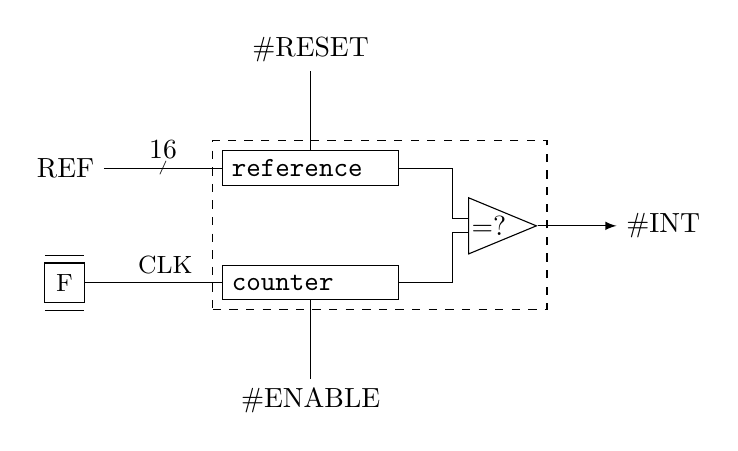
\begin{tikzpicture}[>=latex]
\coordinate (center) at (0,0);
\node[draw, text width = 2cm, above = 0.5 cmof center] (reference) {\texttt{reference}};
\node[draw, text width = 2cm, below = 0.5cm of center] (counter) {\texttt{counter}};
\node[draw, text width = 0.4cm, right = 2cm of center, shape = isosceles triangle, inner sep=1dd] (comparator) {=?};
\node[right = of comparator] (int) {\#INT};
\node[above = of reference] (reset) {\#RESET};
\node[below = of counter] (enable) {\#ENABLE};
\node[left = 1.5cm of reference] (ref-input) {REF};
\node[left = 0.25cm of counter.north west] (clk) {\small{CLK}};

% draw a quartz
\coordinate (quartz) at ([xshift = -2cm]counter.west);
 \node[]  at (quartz) {\small{F}};
\draw (quartz) ++(-0.25,0.25) rectangle ++(0.5,-0.5);
\draw (quartz) ++(-0.25,0.35) -- ++ (0.5,0);
\draw (quartz) ++(-0.25,-0.35) -- ++ (0.5,0);
\draw (reset) -- (reference);
\draw (enable) -- (counter);

% draw wires
\draw (reference.east) -| ([xshift = -0.2cm]comparator.160) -- (comparator.160);
\draw (counter.east) -| ([xshift = -0.2cm]comparator.200) -- (comparator.200);
\draw (ref-input) -- (reference) node[midway] {\tiny{/}} node[midway, above] {16};
\draw (quartz) ++(0.25,0) -- (counter);
\draw[->] (comparator) -- (int);
\node[draw, dashed, fit = (reference) (counter) (comparator)] {};

\end{tikzpicture}

\end{frame}

\begin{frame}{Диаграмма работы}
\centering

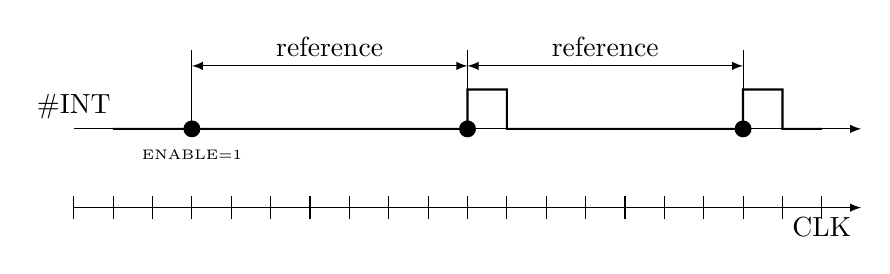
\begin{tikzpicture}[>=latex]
% set clock and #INT time lines
\draw[->] (0,0) -- (10,0) node[pos=0.95, below] {CLK};
\draw[->] (0,1) -- (10,1) node[pos=0.0, above] {\#INT};

\foreach \x in { 0, 1, 2, 3, 4, 5, 6, 7, 8, 9, 10, 11, 12, 13, 14, 15, 16, 17, 18, 19} {
    \draw (\x/2,-0.15) -- (\x/2,0.15)  {};
    \coordinate (tick\x) at (\x/2, 1);
};

\draw[fill=black] (tick3) circle (0.1cm);
\node[below = 0.15cm of tick3] (event-enable) {\tiny{ENABLE=1}};

\draw[fill=black] (tick10) circle (0.1cm);
\draw[fill=black] (tick17) circle (0.1cm);
\draw (tick3)  -- ++(0, 1);
\draw (tick10) -- ++(0, 1);
\draw (tick17) -- ++(0, 1);
\draw[<->] ([yshift=0.8cm]tick3) -- ([yshift=0.8cm]tick10) node[midway, above] {reference};
\draw[<->] ([yshift=0.8cm]tick10) -- ([yshift=0.8cm]tick17) node[midway, above] {reference};

% The actual #CLK plot
\draw[thick] (tick1) -- (tick10) -- ++(0, 0.5) -- ++(0.5, 0) --
            (tick11) -- (tick17) -- ++(0, 0.5) -- ++(0.5, 0) -- (tick18) -- (tick19);

\end{tikzpicture}    
\end{frame}

\begin{frame}[fragile]{Моделирование с фиксированным шагом}

\begin{verbatim}
on_clk() {
  if (enable) counter +=1;
  if (counter == reference) {
      raise_int();
      counter = 0;
  } else {
      lower_int();
  }
}

on_reset() {
    reference = 0;
    counter = 0;
}
\end{verbatim}    
\end{frame}

\begin{frame}{Типичные значения параметров таймера}

\begin{itemize}
    \item $\mathsf{F} \approx 10\ \text{МГц}$
    \item $\mathsf{reference} > 10^3$
    \item \#RESET — не чаще одного раза в $\approx$ 100 секунд
\end{itemize}

$\Rightarrow$ внешне видимый эффект (\#INT) происходит примерно один раз в $10^3$ тактов.
    
\end{frame}

\begin{frame}{Оптимизация}
Не моделировать внешне ненаблюдаемые действия.

\centering
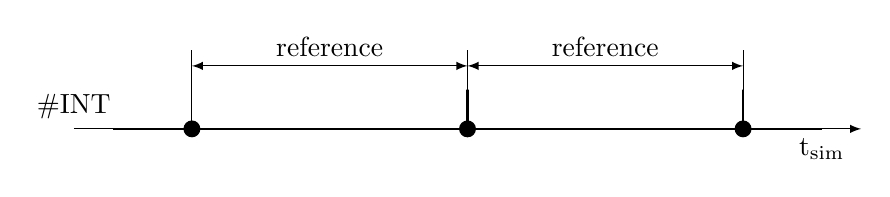
\begin{tikzpicture}[>=latex]
% set clock and #INT time lines
\draw[->] (0,1) -- (10,1) node[pos=0.0, above] {\#INT} node[pos=0.95, below] {t\textsubscript{sim}};

\foreach \x in { 0, 1, 2, 3, 4, 5, 6, 7, 8, 9, 10, 11, 12, 13, 14, 15, 16, 17, 18, 19} {
    \coordinate (tick\x) at (\x/2, 1);
};

\draw[fill=black] (tick3) circle (0.1cm);

\draw[fill=black] (tick10) circle (0.1cm);
\draw[fill=black] (tick17) circle (0.1cm);
\draw (tick3)  -- ++(0, 1);
\draw (tick10) -- ++(0, 1);
\draw (tick17) -- ++(0, 1);
\draw[<->] ([yshift=0.8cm]tick3) -- ([yshift=0.8cm]tick10) node[midway, above] {reference};
\draw[<->] ([yshift=0.8cm]tick10) -- ([yshift=0.8cm]tick17) node[midway, above] {reference};

% The actual #CLK plot
\draw[thick] (tick1) -- (tick10) -- ++(0, 0.5) -- ++(0, -0.5) --
            (tick11) -- (tick17) -- ++(0, 0.5) -- ++(0, -0.5) -- (tick18) -- (tick19);
\end{tikzpicture}

\end{frame}

\begin{frame}[fragile]{Моделирование событий}
\begin{verbatim}
struct event_t {
    time_t delta;
    dev_t *device;
    (*function)();
}
event_t event_queue[100];
time = 0;
foreach e in event_queue {
    e.function(e.device);
    time +=e.delta;
}
\end{verbatim}

\end{frame}

\section{Отложенный ответ}

\begin{frame}{Пример №2: ожидание ответа}

\begin{center}
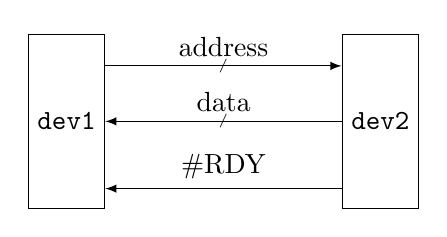
\begin{tikzpicture}[>=latex]
\node[draw, inner ysep=1cm] (dev1) {\texttt{dev1}};
\node[draw, inner ysep=1cm, right= 3cm of dev1] (dev2) {\texttt{dev2}};

\draw[->] (dev1.55) -- (dev2.125) node[midway] {\tiny{/}} node[midway, above] {address};

\draw[->] (dev2) -- (dev1) node[midway] {\tiny{/}} node[midway, above] {data};

\draw[->] (dev2.240) -- (dev1.300) node[midway, above] {\#RDY};
\end{tikzpicture}                 \end{center}

\begin{enumerate}
    \item Запрос от \texttt{dev1}: address.
    \item \texttt{dev2} вычисляет data.
    \item \texttt{dev2} оповещает \texttt{dev1} о готовности данных \textit{через некоторое время} $\Delta T$ с помощью \#RDY.
    \item \texttt{dev1} после отправки address и до получения \#RDY работает независимо.
\end{enumerate}

\end{frame}

\begin{frame}{Реализация}

\texttt{dev1:}
\begin{enumerate}
    \item dev2.read(address)
\end{enumerate}
\texttt{dev2:}
\begin{enumerate}
    \item data = get_data(address)
    \item event_queue.post($\Delta T$, dev1, rdy())
\end{enumerate}
\texttt{dev1:}
\begin{enumerate}
    \item rdy(): чтение data.
\end{enumerate}

\end{frame}

\section{Теория}

\begin{frame}{Очередь событий}
\centering

\begin{tikzpicture}[>=latex, font=\scriptsize]
    \draw[->] (0,0) -- (10,0) node[pos=0.9, below] (sim-time) {Время};

    \foreach \x in { 1, 2, 3, 4, 5, 6, 7, 8, 9} {
        \draw (\x,-0.15) -- (\x,0.15) node (tick\x) {};
    };
    \node[shape=dart, draw, shape border rotate=270 ] at (2, 0.5) (currevent) {};
    \node[draw, arrow box, arrow box arrows={north:.7cm}, text width=2.5cm, align=center, below = 0cm of currevent] (tsim) {Текущее симулируемое время};
    \node[align=center, above=0.2cm of currevent, text width=2cm]  {Обрабатываемое событие};

    \node[shape=dart, draw, shape border rotate=270 ] at (5, 0.5) (futureevent) {};
    \node[align=center, above=0.2cm of futureevent, text width=2cm] {Запланированное событие};

    \node[fill=black!10, shape=dart, draw, shape border rotate=270 ] at (7, 0.5) (newbornevent) {};
    \node[align=center, above=0.2cm of newbornevent, text width=1.5cm] {Новое событие};

    \node[shape=dart, draw, shape border rotate=270 ] at (9, 0.5) (futureevent2) {};
    \node[shape=dart, draw, shape border rotate=270, above=0cm of futureevent2 ] (futureevent3) {};

    \draw[dashed, ->] (currevent.south) .. controls +(1,-0.5) and +(-1,-0.5) .. (newbornevent.south); % node[below, pos=0.7, text width=3cm] {Обработка события порождает новое событие в будущем};

    \end{tikzpicture}

\end{frame}

\begin{frame}{Содержимое и результаты}
Что содержится в одном событии:
\begin{itemize}
    \item функция, которая должна быть вызвана,
    \item объект, состояние которого изменяется.
\end{itemize}

Результаты обработки события:
\begin{itemize}
    \item изменение состояния системы,
    \item добавление/уничтожение событий.
\end{itemize}

\end{frame}

\begin{frame}{Вопросы}
Что будет происходить с очередью событий при
\begin{enumerate}
    \item записи в \texttt{reference} или \#RESET?
    \item выключении таймера (ENABLE ← 0)?
    \item чтении регистра \texttt{counter}?
\end{enumerate}

\end{frame}


\begin{frame}[fragile]{Алгоритм DES}

\begin{verbatim}
struct event_t {
    time_t delta;
    dev_t *device;
    (*function)();
}
uint sim_time = 0;
while (! empty(queue)) {
    sim_time += get_delta(queue);
    evt_t evt = pop(queue);
    evt.fn(evt.device, queue);
}
\end{verbatim}

\end{frame}

% \begin{frame}{Свойства событий}
% 
% \begin{itemize}
% \item Порождаемые события не могут попасть в прошлое.
% \item Обработка событий может не только порождать события в будущем, но и отменять некоторые из них (ещё не обработанные).
% \item Несколько событий могут иметь одинаковую метку времени.
% \end{itemize}
% 
% \end{frame}

\section{Практический пример}

\begin{frame}[fragile]{Пример на модели \texttt{or1k}}
\emph{Демо}

\begin{verbatim}
simics> log-level 1
New global log level: 1
simics> continue-cycles 199
[chip0] v:0x031c p:0x031c  nop
simics> peq
  Step  Object      Description

 Cycle  Object      Description
     1  tick0       reference_reached
499802  cosim_cell  sync_report
999801  sim         Time Quantum End
999801  cosim_cell  sync_block
\end{verbatim}

\end{frame}

\section{Два класса моделей}

\begin{frame}{На этой лекции}
\begin{itemize}
    \item Совместная работа с моделью процессора.
    \item Работа с несколькими процессорами сразу.
\end{itemize}
\end{frame}

\section{Косимуляция}

\begin{frame}{Какие типы моделей нам известны}

\begin{itemize}
    \item Интерпретация\pause: процессоры. \pause
    \item Очередь событий\pause: таймер.\pause
    \item «Мгновенная» модель «стимул — отклик»\pause: ОЗУ.
\end{itemize}

\end{frame}

\begin{frame}{Модель многопроцессорной системы}
\begin{tikzpicture}[>=latex]

\node[draw, circle] (core1) {Ядро 1};
\node[draw, circle, right = of core1] (core2) {Ядро 2};
\node[draw, circle, right = of core2] (core3) {Ядро 3};
\node[draw, circle, right = of core3] (core4) {Ядро $N$};

\coordinate[below = 2.3cm of core1] (c3);
\coordinate[below = 1.5cm of core4] (c4);

\node[draw, fit = (c3) (c4), inner ysep=1pt ] (shmem) {Общая память};

\draw[<->] (core1.south) -- (shmem);
\draw[<->] (core2.south) -- (shmem);
\draw[<->] (core3.south) -- (shmem);
\draw[<->] (core4.south) -- (shmem);

\end{tikzpicture}

\end{frame}

\begin{frame}[fragile]{Квотированная симуляция}
\begin{tikzpicture}[>=latex]
\draw[->] (0,0) -- (8,0) node[pos=0.9, below] (sim-time) {Физическое время};

\foreach \x in { 1, 2, 3, 4, 5, 6, 7} {
    \draw (\x,-0.15) -- (\x,0.15) node (tick\x) {};
};
\matrix[anchor=south west] at (-0.5,0.5){
    \node[] {CPU3}; & & & \node[shape=single arrow, draw, text width = 2cm, inner xsep = 0cm, fill=black!5] (arr3) {}; \\
    \node {CPU2}; & & \node[shape=single arrow, draw, text width = 2cm, inner xsep = 0cm, fill=black!10] (arr2) {}; & \\
    \node {CPU1}; & \node[shape=single arrow, draw, text width = 2cm, inner xsep = 0cm, fill=black!15] (arr1) {}; & & \\
};

\draw[->] (arr1.east) -- (arr2.west);
\draw[->] (arr2.east) -- (arr3.west);

\end{tikzpicture}

\end{frame}

\begin{frame}[fragile]{Квотированная симуляция}

    \begin{tikzpicture}[>=latex]
        \draw[->] (0,0) -- (8,0) node[pos=0.9, below] (sim-time) {Симулируемое время};

    \foreach \x in { 1, 2, 3, 4, 5, 6, 7} {
        \draw (\x,-0.15) -- (\x,0.15) node (tick\x) {};
    };
    \matrix[anchor=south west] at (-0.5,0.5){
        \node {CPU3}; & \node[shape=single arrow, draw, text width = 2cm, inner xsep = 0cm, fill=black!5] (arr3) {};  \\
        \node {CPU2}; & \node[shape=single arrow, draw, text width = 2cm, inner xsep = 0cm, fill=black!10] (arr2) {}; \\
        \node {CPU1}; & \node[shape=single arrow, draw, text width = 2cm, inner xsep = 0cm, fill=black!15] (arr1) {}; \\
    };

    % \draw[->] (arr1.east) -- (arr2.west);
    % \draw[->] (arr2.east) -- (arr3.west);

    \end{tikzpicture}

\end{frame}

\begin{frame}{Размер квоты}
\begin{itemize}
\item  Процессор может исполнить меньше инструкций, чем содержится в выданной ему квоте.
\item Не следует увлекаться излишне большими квотами, пытаясь ускорить исполнение.
\item В DES-модели могут быть реализованы псевдо-события, обработка которых вызывает переключение текущего процессора.
\end{itemize}

\end{frame}

\begin{frame}{Совместная симуляция DES и исполняющей модели}
\centering
    \begin{tikzpicture}[>=latex, font=\scriptsize]

    \draw[->] (-0.5,0) -- (10.5,0); % node[pos=0.9, above] (sim-time) {Время};

    \begin{scope}
    \clip (0,-2) rectangle (10, 2.5);
    \foreach \x in { 1, 2, 3, 4, 5, 6, 7, 8, 9} {
        \draw (\x,-0.15) -- (\x,0.15) node (tick\x) {};
    };

    \node[shape=dart, draw, shape border rotate=270 ] at (1, 0.5) (event1) {};
    \node[shape=dart, draw, shape border rotate=270 ] at (5, 0.5) (event2) {};
    \node[shape=dart, draw, shape border rotate=270 ] at (9, 0.5) (event3) {};

    \node[above of=event2] (desalabel) {Дискретные события};
    \draw[->] (desalabel) -- (event1);
    \draw[->] (desalabel) -- (event2);
    \draw[->] (desalabel) -- (event3);

    \draw (3,-0.5) ellipse[x radius = 2cm, y radius = 0.5cm] node {Исполнение процессора} ;
    \draw (7,-0.5) ellipse[x radius = 2cm, y radius = 0.5cm] node {Исполнение процессора} ;

    \draw (-1,-0.5) ellipse[x radius = 2cm, y radius = 0.5cm] node {} ;
    \draw (11,-0.5) ellipse[x radius = 2cm, y radius = 0.5cm] node {} ;
    \end{scope}
    \end{tikzpicture}

\end{frame}

\begin{frame}{Косимуляция}

\centering
    \begin{tikzpicture}[>=latex]
    \node[draw, circle, text width = 3cm, text badly centered] (dessim) {Симулятор дискретных событий};
    \node[draw, circle, text width = 3cm, text badly centered, right = 2.5cm of dessim] (execsim) {Модель исполняющего устройства};

    \draw (dessim.45)   edge[bend left = 45, ->] (execsim.135);
    \node[above=1cm of execsim.135] {\small Длительность до следующего события};
    \draw (execsim.225) edge[->, bend left = 45] (dessim.315);
    \node[below=1cm of dessim.315] {\small Число исполненных шагов};

    \end{tikzpicture}

\end{frame}

\section{Практический пример}

\begin{frame}[fragile]{Пример на модели \texttt{viper-busybox.simics}}
Квота на восьмиядерной конфигурации:
\begin{verbatim}
simics> cpu-switch-time
Current time quantum:     0.0001 s
  200000.0  viper.mb.cpu0.core[0][0]
  200000.0  viper.mb.cpu0.core[0][1]
  200000.0  viper.mb.cpu0.core[1][0]
  200000.0  viper.mb.cpu0.core[1][1]
  200000.0  viper.mb.cpu0.core[2][0]
  200000.0  viper.mb.cpu0.core[2][1]
  200000.0  viper.mb.cpu0.core[3][0]
  200000.0  viper.mb.cpu0.core[3][1]
Default time quantum not set yet
\end{verbatim}

\end{frame}

\begin{frame}[fragile]{Пример на модели \texttt{viper-busybox.simics}}
Симулируемое время на восьмиядерной конфигурации:
\begin{verbatim}
simics> ptime -all
processor                      steps      cycles  time [s]
viper.mb.cpu0.core[0][0]  4602030000  5134030000     2.567
viper.mb.cpu0.core[0][1]  4925600000  5134000000     2.567
viper.mb.cpu0.core[1][0]  4925600000  5134000000     2.567
viper.mb.cpu0.core[1][1]  4925600000  5134000000     2.567
viper.mb.cpu0.core[2][0]  4925600000  5134000000     2.567
viper.mb.cpu0.core[2][1]  4925600000  5134000000     2.567
viper.mb.cpu0.core[3][0]  4925600000  5134000000     2.567
viper.mb.cpu0.core[3][1]  4925600000  5134000000     2.567
\end{verbatim}
    
\end{frame}

\section{Заключение}
\begin{frame}{Дополнительные вопросы DES}
\begin{itemize}
    \item Совместная работа с моделью процессора.
    \item Работа с несколькими процессорами сразу.
    \item Сценарии, когда действительно надо моделировать каждый такт.
\end{itemize}
\end{frame}

\begin{frame}{Статьи для перевода}
\url{https://github.com/yulyugin/ilab-simics/wiki/translation-list}
\begin{itemize}
    \item План статьи (описание всех секций).
    \item Минимум 10000 символов.
    \item Дедлайн — 31 декабря 2014 г.
\end{itemize}
\end{frame}

\section{Литература}

\begin{frame}[allowframebreaks]{Литература}
\begin{thebibliography}{99}
    \bibitem{patterson} Паттерсон Д., Хеннесси Дж. Архитектура компьютеров и проектирование компьютерных систем — СПб.: Питер — 2011 — 784~с. — ISBN 978-5-459-00291-1
    \bibitem{sim-handbook} Handbook of Simulation. Principles, Methodology, Advances, Applications, and Practice / ed. by J. Banks. — John Wiley \& Sons, Inc., 1998. — ISBN 0-471-13403-1. — \url{http://books.google.com/books?id=dMZ1Zj3TBgAC} % http://lib.mipt.ru/book/288185/
    \bibitem{simics-processor-integration} Wind River. Simics Processor Integration Guide.
\end{thebibliography}
\end{frame}

\section{Конец}
% The final "thank you" frame
\begin{frame}

{\huge{Спасибо за внимание!}\par}

\vfill

Слайды и материалы курса доступны по адресу \url{http://is.gd/ivuboc} % http://atakua.doesntexist.org/wordpress/simulation-course-russian/

\vfill

\tiny{\textit{Замечание}: все торговые марки и логотипы, использованные в данном материале, являются собственностью их владельцев. Представленная точка зрения отражает личное мнение автора.
Материалы доступны по лицензии Creative Commons Attribution-ShareAlike (Атрибуция — С сохранением условий) 4.0 весь мир (в т.ч. Россия и др.). Чтобы ознакомиться с экземпляром этой лицензии, посетите \url{http://creativecommons.org/licenses/by-sa/4.0/}
}

\end{frame}


\end{document}
